
% % % % % % % % % % % % % % % % % %
%DGL 1. Ordnung
% % % % % % % % % % % % % % % % % %	
\begin{tabularx}{\textwidth}{|p{100pt}|p{100pt}|X|}
\hline
\rowcolor{Gray}
\multicolumn{3}{|c|}{\textbf{DGL 1. Ordnung} \qquad \fb{S.554}}\\
\hline
%	Art & Form & Lösung\\
%	\hline
	Separation \newline
	\fb{S.555 (9.1.1.2)}&
	$y' = f(x)\cdot g(y)$&
	$\begin{aligned}[t]
		y^{\prime} &=f(x) \cdot g(y) \quad &|& \ : g(y) \neq 0 ! ! ! \\
		y^{\prime} &=f(x) \quad &|& \ \int_{x_{0}}^{x}(\ldots) d \tilde{x} \\ \int_{x_{0}}^{x} \frac{y^{\prime}(\tilde{x})}{g(y(\tilde{x}))} d \tilde{x} &=\int_{x_{0}}^{x} f(\tilde{x}) d \tilde{x} \quad &|& \ d y=y^{\prime}(\tilde{x}) d \tilde{x}\\ \int_{y_{0}=y\left(x_{0}\right)}^{y(x)} \frac{1}{g(y)} d y &=\int_{x_{0}}^{x} f(\tilde{x}) d \tilde{x} &\rightarrow& \ \text{Aufl"osen} \rightarrow \text{Gleichung in} \ x, y\\
	 \end{aligned}$ \\
\hline
	Linearterm&
	$y^{\prime}=f(a x+b y+c)$&
	$\begin{aligned}[t]
		y^{\prime} &=f(a x+b y+c) \quad &|& \ \text{Substitution: } z = ax+bx+c\\ 
		y^{\prime} &=f(z) \quad &|& \ \text{differenzieren} \quad z^{\prime}=a+b y^{\prime}\\ 
		z^{\prime} &=a+b y^{\prime} \quad &|& \ y^{\prime}=f(z) \\ 
		z^{\prime} &=(a+b \cdot f(z)) \cdot 1 \Rightarrow && \text{separiert! Anfangsbedingungen: }  z_{o}=a x_{0}+b y_{0}+c\\
	\end{aligned}$\\
\hline
	Gleichgradigkeit&
	$y'=f\left(\dfrac{y}{x}\right)$ &
	$\begin{aligned}[t]
		y^{\prime} &=f\left(\frac{y}{x}\right) \quad
		&|& \text { Substitution: } \quad z=\frac{y}{x} \quad \Leftrightarrow \quad y=z \cdot x \quad(x \neq 0)\\ 
		y^{\prime} &=f(z) \quad &|& 
		\text { differenzieren: } \quad y^{\prime}=z+z^{\prime} \cdot x\\ 
		y^{\prime} &=z+z^{\prime} \cdot x \quad &|& \ y^{\prime}=f(z)\\ 
		f(z) &=z+z^{\prime} \cdot x \quad &|& \ \text{umformen}\\
		z^{\prime}&=(f(z)-z) \cdot \frac{1}{x} &\Rightarrow& \text { separiert! } \quad \text { Anfangsbedingungen: } \quad z_{o}=\frac{y_{0}}{x_{0}}\\
	\end{aligned}$\\
\hline
	Allgemeine DGL \newline 1. Ordnung&
	$y'+f(x)y = g(x)$\newline\newline
	$y_{o}=y(x_{0})$ \newline
	$g(x)$ : Störterm&
%	$\begin{array}{ll}
%		y=e^{-\int f(x) dx}(k+\int g(x)e^{\int f(x)dx}dx) & \qquad (k\in\mathbf{R}) \quad \text{ Var. } k \text{ ist Konstante }\\
%		Y=y_H+y_p \quad &
%	\end{array}$
	\begin{minipage}{0.5\textwidth}
		\vspace{1mm}
		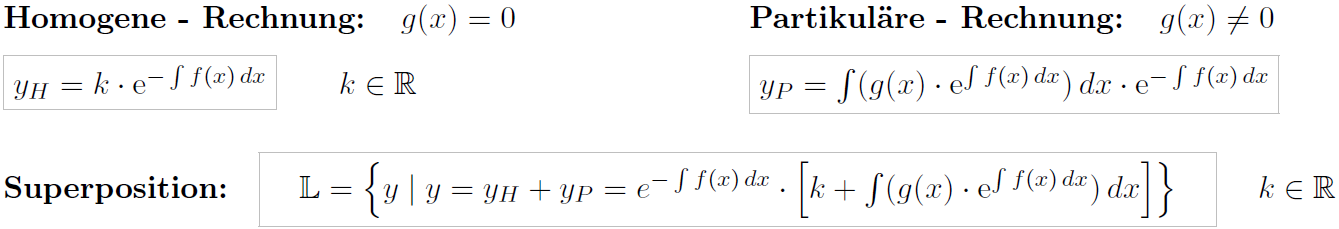
\includegraphics[width = 1.18\textwidth]{bilder/alg_DGL1.png}
	\end{minipage}
	\\
	\hline

\end{tabularx}	
\end{center}
\end{table}	